\documentclass[11pt]{article}
%%
%% Package includes to provide the basic style
%%
\usepackage[top=3.5cm, bottom=3.5cm, left=2.5cm, right=2.5cm]{geometry}
\usepackage{hyperref}
\usepackage{pdfpages}
\usepackage{algorithm2e}
\usepackage[authoryear]{natbib}
\bibliographystyle{plainnat}
\usepackage{appendix}
\usepackage{pgfplotstable}
\usepackage[font={color=darkgray,footnotesize, sf, it}]{caption}
\usepackage{amsmath}
\usepackage{helvet}
\usepackage{wrapfig}
\usepackage{multicol}
\usepackage[eulergreek]{sansmath}
\usepackage{listings}
\usepackage{setspace}
\usepackage{graphicx}
\usepackage{longtable}
\usepackage{minted}
\usepackage{relsize}
\linespread{1.2}
\lstset { %
    language=C++,
    backgroundcolor=\color{black!5}, % set backgroundcolor
    basicstyle=\ttfamily\footnotesize,% basic font setting
}
\usepackage{bchart}
\usepackage{booktabs}
\usepackage{xcolor}

\definecolor{skyblue}{RGB}{203,240,255}
\definecolor{forestgreen}{RGB}{0,96,50}
\definecolor{indigo}{RGB}{4,87,239}
\definecolor{darkindigo}{RGB}{1,40,112}
\definecolor{darkpurple}{RGB}{32,14,104}
\definecolor{apple}{RGB}{0,158,13}
\definecolor{bad}{RGB}{239,55,55}
\definecolor{badtoavg}{RGB}{247,128,98}
\definecolor{avg}{RGB}{255,218,117}
\definecolor{avgtogood}{RGB}{190,247,140}
\definecolor{good}{RGB}{102,226,102}

\setlength{\parindent}{0em}
\setlength{\parskip}{1em}
\setlength\parindent{0pt}

\usepackage{titling}
\usepackage{titlesec}
\pretitle{\Huge\bfseries}
\posttitle{\par}

\titlespacing\section{0pt}{12pt plus 4pt minus 2pt}{0pt plus 2pt minus 2pt}
\titlespacing\subsection{0pt}{12pt plus 4pt minus 2pt}{0pt plus 2pt minus 2pt}
\titlespacing\subsubsection{0pt}{12pt plus 4pt minus 2pt}{0pt plus 2pt minus 2pt}

\usepackage[english]{babel}
\usepackage[utf8]{inputenc}
\usepackage{fancyhdr}
 
\pagestyle{fancy}
\fancyhf{}
\rhead{cjd47}
\lhead{CM30141: \textit{Theory of Human-Computer Interaction}}
\cfoot{\thepage} 
\renewcommand{\headrulewidth}{1pt}
\renewcommand{\footrulewidth}{1pt}

\newcommand\wordcount[1]{
\vfill
\textit{Word count: {#1} words (not inc. Citations, Figures or References)}}

\newcommand\essaytitle[1]{
\begin{LARGE}
\textbf{{#1}} \\
\end{LARGE}}

\newcommand\sectiontitle[1]{
\begin{large}
\textbf{{#1}} \medskip \\ 
\end{large}}

%%
%% END OF DEFINITIONS
%%

\begin{document}
\essaytitle{Critical Review: Improving the Efficacy of Games for Change Using Personalization Models}
Persuasion is the act of influencing or reinforcing certain attitudes and behaviours \citep{khaled2008}. The use of technology for encouraging behavioural change to benefit its users or the wider community is a long-term area of research \citep{fogg2002}. This review will present a summary and critical analysis of \citet{orji2017} whose paper explores the use of personalisation models as a persuasive device for improving the efficacy of games which are designed to change user behaviour, as well as putting forward a set of suggestions for future work in this domain of Persuasive Technology.

\sectiontitle{Summary of Contributions}
\citet{orji2017} highlight the rising prominence of \textit{games for change}\footnote{An annual festival exists for workshops and design classes on games for change: \url{www.gamesforchange.org}} that are designed for purposes other than entertainment, to effectively educate players about certain topics in a way that influences their behaviour \citep{busch2015}.  The authors raise the issue that many such games are designed with a ``\textit{one size fits all}'' philosophy whereby the design of the game itself (and its adopted persuasive \textit{strategies}) are not tailored to the \textit{type} of the player. \citet{orji2017} therefore seek to answer two main research questions to understand the observed efficacy of certain strategies in existing games \citep{peng2009,kaipainen2012}. Firstly, whether tailoring games for change to a specific player type increases their persuasiveness. Secondly, if beneficial effects of tailoring are observed, whether these effects are mediated by an improved play experience. If these could be answered, results could inform the future decisions of games designers in which persuasive strategies they adopt to maximise efficacy in certain player types. 

Treating user groups in a monolithic way is generally considered dangerous, especially in the domain of games for health \citep{berkovsky2010}.  To further justify the need to investigate tailoring, the authors then reviewed the persuasive strategies adopted in a range of existing domains of games for change: healthy eating \citep{kaipainen2012, orji2013b}, physical activity \citep{fujiki2008} and disease management \citep{brownson2007}. The authors, by their own admission, comment that this list is by no means exhaustive which gives plenty of scope for future research in other domains.

Initial work by the authors indicated that a strategy shown as effective for one type of gamer could be detrimental to another \citep{orji2013a} (Table \ref{tbl:orji2017-beta-sem}). This table sets out a well-founded taxonomy which maps 7 gamer types defined by the BrainHex model of \citet{nacke2014} (Achiever, Conqueror, Daredevil, Mastermind, Seeker, Socializer and Survivor) against 8 commonly adopted persuasive strategies selected by \citet{gerling2014} based on a large-scale online survey of 1108 gamers.  Participants responded to indicate how likely each of 10 selected strategies (explained through storyboards) would influence eating decisions, using a validated scale \citep{drozd2012} before completing the BrainHex questionnaire to indicate their gamer type. After careful statistical analysis (Exploratory Factor Analysis and PLS-SEM modelling) 8 strategies were chosen which were pairwise distinct. The data collected from this initial experiment therefore forms as valid justification for the later comparison between Achievers (motivated by Reward) and Conquerors (motivated by Competition). 

\begin{table}[H]
\centering
\caption{$\beta$ values confusion matrix: Strength of motivation of different players that result from different strategies. Positive $\beta$ values indicate that gamers of this type are motivated by the corresponding given strategy. Negative $\beta$ values indicate demotivation, whilst an empty value indicates neither motivation nor demotivation \protect\citep{orji2013a}.
}\label{tbl:orji2017-beta-sem}
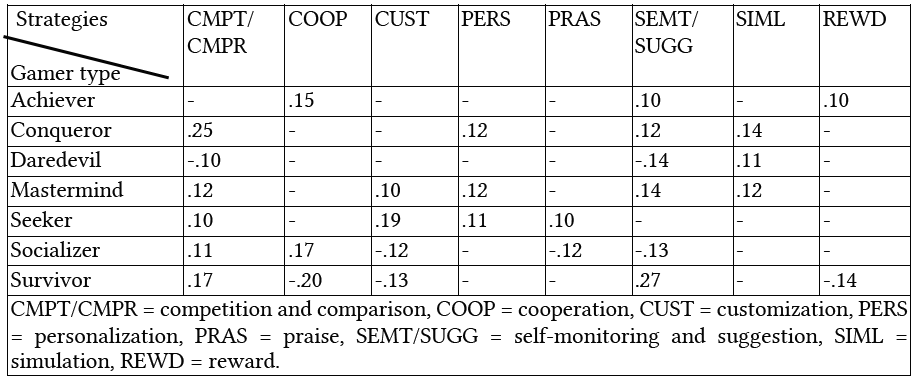
\includegraphics[width=0.75\textwidth]{img/orji2017-beta-sem.png} 
\end{table}

As a way of empirically evaluating this model, the authors focus on the domain of games for healthy eating for illustrative purposes and restrict their considerations towards the effects of two persuasive strategies (Competition and Reward) on two types of gamers (Achiever and Conqueror). Whilst somewhat limiting, this approach allowed scope for direct pairwise comparison between two types of gamers that have been shown empirically to be significantly-distinct in their response to these strategies \citep{orji2013a}. Further, these strategies are also common to existing games \citep{bell2006}. 

To evaluate their research questions, \citeauthor{orji2017} implemented two versions of a custom model-driven online game based on Space Invaders called \textit{Junk Food Aliens} (Figure \ref{fig:orji2017-junk-food-aliens}) which targets the domain of healthy eating - players control an avatar and search for fruits and vegetables to save the planet from an invasion of junk foods. The reward-based version (JFA-R) adopted persuasive strategies such as achievement badges (Figure \ref{fig:orji2017-junk-food-aliens-reward}) whereas the competition-based version (JFA-C) adopted comparative strategies such as leaderboards (Figure \ref{fig:orji2017-junk-food-aliens-competition}). A large-scale randomized controlled study of 272 valid participants (50\% Achievers and 50\% Conquerors) was carried out to investigate the effects of tailoring and contra-tailoring on these two types of gamer. 

\begin{figure}[H]
\centering
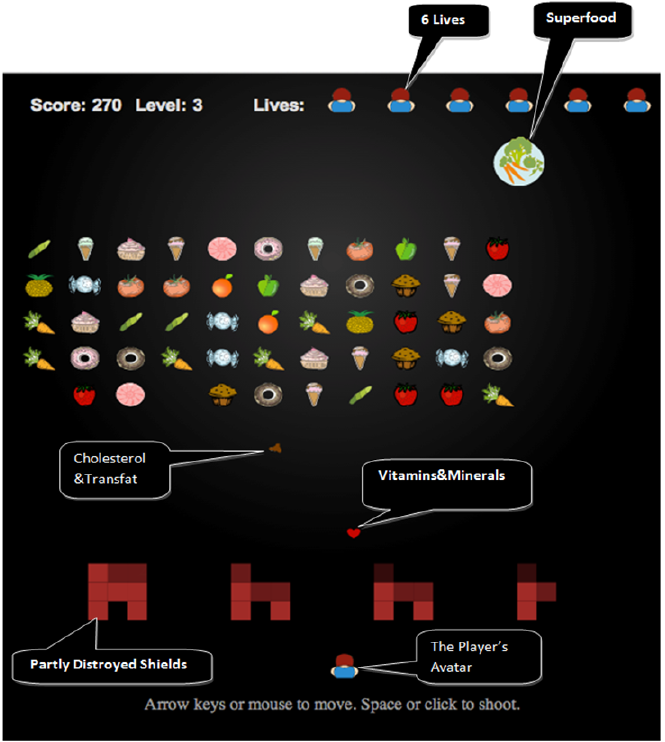
\includegraphics[width=0.4\textwidth]{img/orji2017-junk-food-aliens.png} 
\caption{``Junk Food Aliens'' (JFA): A persuasive game designed to change gamer behaviour towards healthy eating.}\label{fig:orji2017-junk-food-aliens}
\end{figure}

\begin{figure}[H]
\minipage{0.5\textwidth}
\centering
  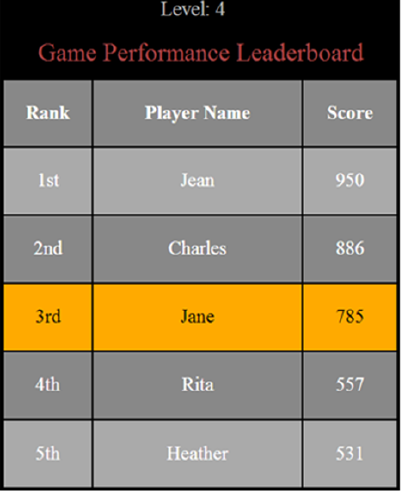
\includegraphics[height=4cm]{img/orji2017-junk-food-aliens-competition.png}
  \caption{JFA-C: Competition-based version of JFA.}\label{fig:orji2017-junk-food-aliens-competition}
\endminipage\hfill
\minipage{0.5\textwidth}%
\centering
  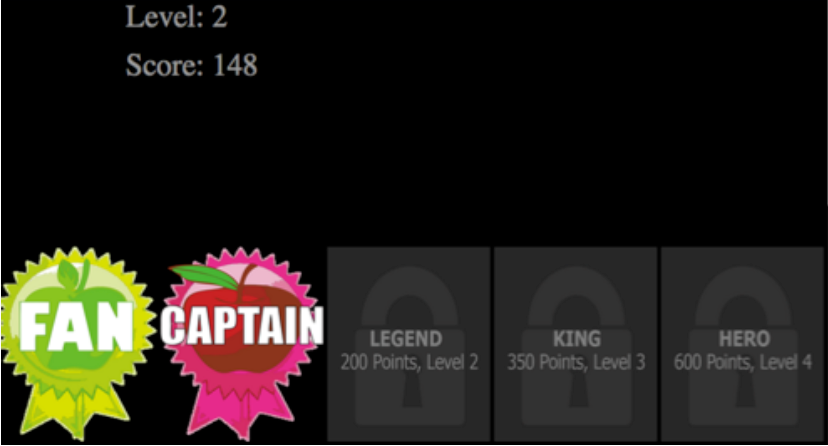
\includegraphics[height=4cm]{img/orji2017-junk-food-aliens-reward.png}
  \caption{JFA-R: Reward-based version of JFA.}\label{fig:orji2017-junk-food-aliens-reward}
\endminipage
\end{figure}

Participants were...

The results showed that tailoring the game to a specific gamer type increased effectiveness (measured by the positive changes in attitudes and intentions towards healthy eating) while contra-tailoring did not.

Main contributions of \citet{orji2017} are therefore fourfold. First, it is important to tailor games for change in order to observe any efficacy as the main experiment demonstrates by measure of change in attitude, self-efficacy, and intention. Second, tailoring can be achieved by modifying the persuasive strategies adopted, rather than the mechanics of the game which will surely minimise the tailoring costs involved. 
Thirdly, the resulting positive effect of tailoring was not seen to be mediated purely by an improved player experience which, if it remained untested, would be a very strong potential confounding factor. Finally, the adoption of a single persuasive strategy is sufficient to observe these effects - combining additional strategies is unpredictable and may be somewhat counter-productive.

\sectiontitle{Justifications for Conclusions}
...

\begin{figure}[H]
\centering
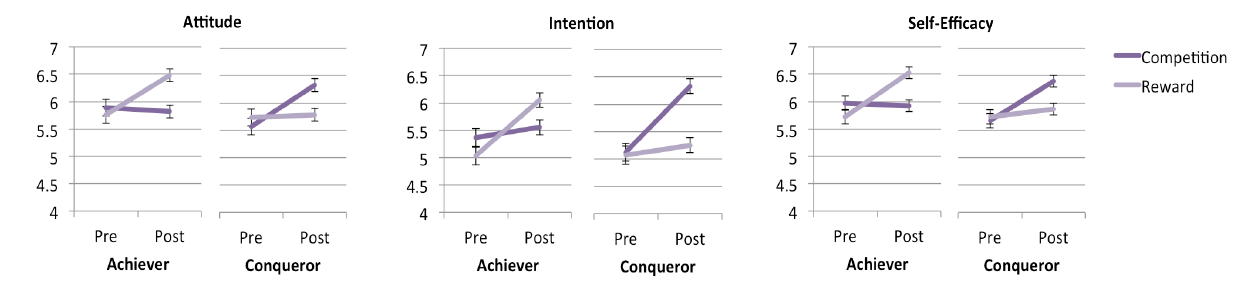
\includegraphics[width=\textwidth]{img/orji2017-tailoring-results.png} 
\caption{Mean values $\pm$ SE for Attitude, Intention, and Self-Efficacy by Gamer type (Achiever, Conqueror) and Game version (Competition, Reward).}\label{fig:orji2017-tailoring-results}
\end{figure}

\begin{figure}[H]
\centering
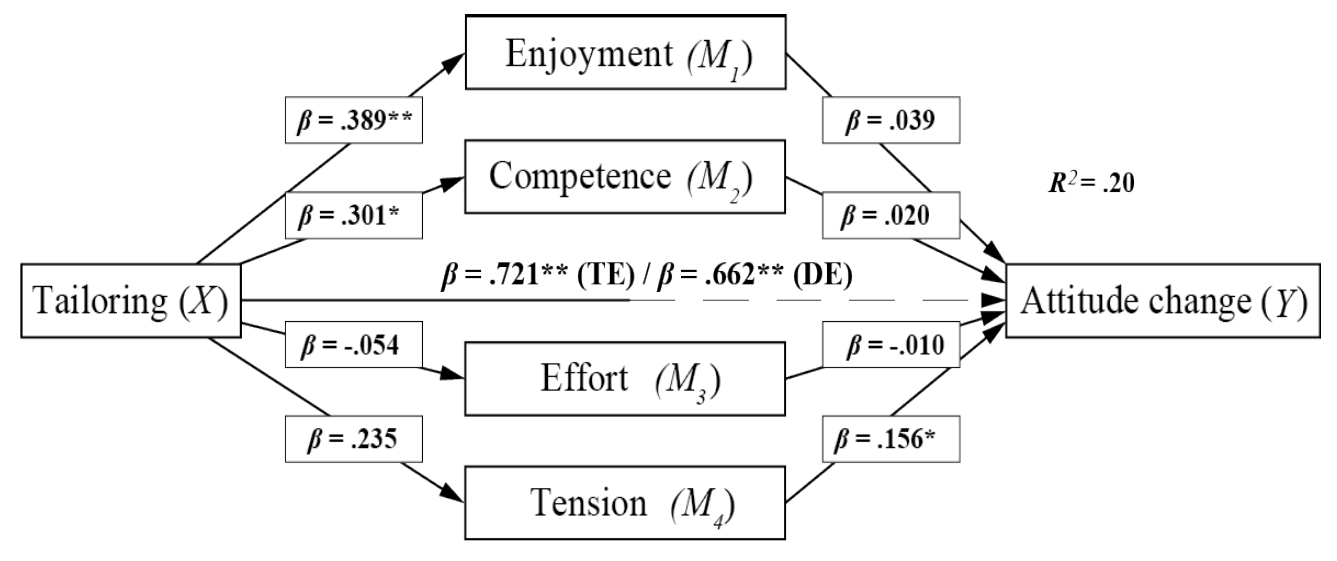
\includegraphics[width=0.75\textwidth]{img/orji2017-tailoring-mediation-results.png} 
\caption{Parallel mediation model of tailoring on attitude change with play experience as mediator.}\label{fig:orji2017-tailoring-mediation-results}
\end{figure}

\sectiontitle{Limitations and Suggested Further Work}
...

\sectiontitle{Conclusion}
...

\wordcount{0}

\newpage
\small
\bibliography{bib1}
\normalsize
\end{document}